% !TEX TS-program = pdflatex
% !TEX encoding = UTF-8 Unicode

\documentclass[a4paper, titlepage=false, parskip=full-, 10pt]{scrartcl}

\usepackage[utf8]{inputenc}
\usepackage[T1]{fontenc}
\usepackage[english, ngerman]{babel}
\usepackage{babelbib}
\usepackage{hyperref}
\usepackage{listings}
\usepackage{framed}
\usepackage{color}
\usepackage{graphicx}
\usepackage[normalem]{ulem}
\usepackage{cancel}
\usepackage{amsmath}
\usepackage{amssymb}
\usepackage{amsthm}
\usepackage{algorithm}
\usepackage{algorithmic}
\usepackage{geometry}
\usepackage{subfigure}
\geometry{a4paper, top=20mm, left=35mm, right=25mm, bottom=40mm}

\newcounter{tasknbr}
\setcounter{tasknbr}{1}
\newenvironment{task}[1]{{\bf Aufgabe \arabic {tasknbr}\stepcounter{tasknbr}} (#1):\begin{enumerate}}{\end{enumerate}}
\newcommand{\subtask}[1]{\item[#1)]}

% Listings -----------------------------------------------------------------------------
\definecolor{red}{rgb}{.8,.1,.2}
\definecolor{blue}{rgb}{.2,.3,.7}
\definecolor{lightyellow}{rgb}{1.,1.,.97}
\definecolor{gray}{rgb}{.7,.7,.7}
\definecolor{darkgreen}{rgb}{0,.5,.1}
\definecolor{darkyellow}{rgb}{1.,.7,.3}
\lstloadlanguages{C++,[Objective]C,Java}
\lstset{
escapeinside={§§}{§§},
basicstyle=\ttfamily\footnotesize\mdseries,
columns=fullflexible, % typewriter font look better with fullflex
keywordstyle=\bfseries\color{blue},
% identifierstyle=\bfseries,
commentstyle=\color{darkgreen},      
stringstyle=\color{red},
numbers=left,
numberstyle=\ttfamily\scriptsize\color{gray},
% stepnumber=5,
% numberfirstline=true,
breaklines=true,
% prebreak=\\,
showstringspaces=false,
tabsize=4,
captionpos=b,
% framexrightmargin=-.2\textwidth,
float=htb,
frame=tb,
frameshape={RYR}{y}{y}{RYR},
rulecolor=\color{black},
xleftmargin=15pt,
xrightmargin=4pt,
aboveskip=\bigskipamount,
belowskip=\bigskipamount,
backgroundcolor=\color{lightyellow},
extendedchars=true,
belowcaptionskip=15pt}

%% Enter current values here: %%
\newcommand{\lecture}{Algorithmische Geometrie SS15}
\newcommand{\tutor}{}
\newcommand{\assignmentnbr}{4}
\newcommand{\students}{Julius Auer, Alexa Schlegel}
%%-------------------------------------%%

\begin{document}  
{\small \textsl{\lecture \hfill \tutor}}
\hrule
\begin{center}
\textbf{Übungsblatt \assignmentnbr}\\
[\bigskipamount]
{\small \students}
\end{center}
\hrule

\begin{task}{Bewegungsplanung in der Ebene}\item[]
Gegeben sei ein kreisförmiger Roboter $R$ mit Radius $d$, sowie eine Menge $H={p_1, \dots, p_n}$ von $n$ punktförmigen Hindernissen in der Ebene. Eingabewerte sind Startpunkt $s$ und Zielpunkt $z$. Die Ausgabe ist kollisionsfreier Weg $w$ (Polygonzug), falls er existiert, sonst $\emptyset$.

Die Idee des Algorithmus ist es, aus $H$ ein Voronio-Diagramm (VD) zu erstellen und das Zentrum des Roboters auf den Voronio-Kanten (VK) entlang zum bewegen. Zusätzlich werden diejenigen VK entfernt, wo der Abstand der zugehörigen Punkte kleiner ist als der Durchmesser des Roboter. Auf den verbleibenden Kanten kann sich der Roboter bewegen, d.h. sein Zentrum bewegt sich.

Der Algorithmus wird in 3 Schritte unterteilt:

{\large\textcircled{\small{1}}} Roboter von $s$ zum/auf VD bewegen\\
{\large\textcircled{\small{2}}} Roboter entlang des VD bewegen\\
{\large\textcircled{\small{2}}} Roboter von VD zu $z$ bewegen\\

\begin{algorithm}
\caption{movingAround($H, s, z, d$)}
\begin{algorithmic}[1]
\STATE Berechnung VD($H$)
\STATE VR($s$) und VR($z$) bestimmen
\IF{$s$ bzw. $z$ kollidieren mit Punkt in VR($s$) bzw. VR($z$)}
		\RETURN{$\emptyset$}
\ENDIF
\STATE $s'$ und $z'$ auf VD finden und als Knoten zu VD($H$) hinzufügen und Kanten aufsplitten (senkrecht vom Punkt in zugehöriger VR wegbewegen bis VK getroffen wird, siehe~Abbildung\ref{fig:vds})
\STATE Sei $G$ der zugehörige Graph zum VD($H$): alle Kanten entfernen, wo der Abstand der zugehörigen Punkte $\leq d$ ist
\IF{Weg $w$ von $s'$ nach $z'$ existiert}
		\RETURN{$w \cup \overline{ss'} \textrm{ und } \overline{pp'}$}
		\ELSE
				\RETURN {$\emptyset$}
\ENDIF
\end{algorithmic}
\end{algorithm}

\begin{figure}[h]
\begin{center}
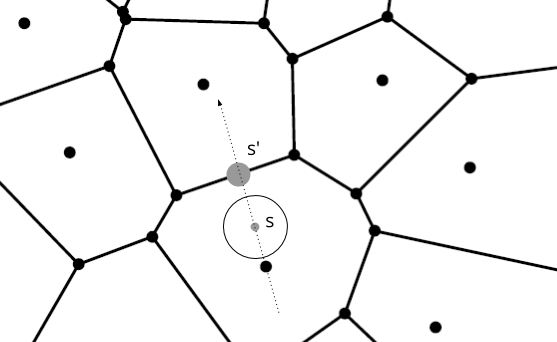
\includegraphics[width=7cm]{vds.png}
\end{center}
\caption{Finden von $s'$}
\label{fig:vds}
\end{figure}

Der existierende Weg kann z.B. per Tiefensuche oder Dijkstra bestimmt werden. Liegt der Start bzw. Endpunkt auf einer Kante die später entfernt wird, so liefert die Suche nach einem existierenden Weg kein Ergebnis.

Was mir noch nicht ganz klar ist, wenn $s$ und $z$ in einer unbeschränkten VR liegen (bzw. man da immer irgendwie hin kommt) dann könnte man doch immer einmal komplett außen rum laufen, oder? Oder ist man in einem Zimmer gefangen wo die Punkte auf dem Boden rumliegen und man sonst gegen die Wand läuft?
\end{task}

\begin{task}{Geometriche Graphen}
\subtask{a}
Induktion über $|V|$:

I.A.: Für $G_0=(V,E,F)$ zusammenhängend und planar mit $|V|=1$ folgt offensichtlich $|E|=0$ und $|F|=1$.

I.V.: Für $G_n=(V,E,F)$ zusammenhängend und planar mit $|V|=n$ gilt: $|E|=|V|+|F|-2$

$n\rightarrow n+1$: Aus $G_{n+1}=(V',E',F')$ zusammenhängend und planar mit $|V'|=n+1$ werden ein Knoten $v$ und alle zu $v$ inzidenten Kanten entfernt.

Fall 1: Der entstehende Graph ist zusammenhängend:\\
Für den entstehenden Graphen $G_n=(V,E,F)$ gilt $|V|=n$ und $|E|=|E'|-deg(v)$ sowie die I.V.. Nun muss $v$ in einer Facette $f$ von $G_n$ liegen und somit jede zu $v$ inzidente Kante in $G_{n+1}$ zu einem Knoten auf dem Rand von $f$ führen (sonst wäre Planarität verletzt). Die zu $v$ inzidenten Kanten unterteilen $f$ offensichtlich in $deg(v)-1$ zusätzliche Facetten. Somit gilt für $G_{n+1}$:
\begin{align*}
F'&=F+deg(v)-1\\
&=|E|-|V|+2+deg(v)-1\\
&=|E'|-deg(v)-|V'|+1+2+deg(v)-1\\
&=|E'|-|V'|+2
\end{align*}

Fall 2: Der entstehende Graph ist nicht zusammenhängend:\\
{\large\textcircled{\small{1}}} Dann entstehen $k\le deg(v)$ planare Zusammenhangskomponenten $G^1,...,G^k$. Für jede gilt die I.V..\\
{\large\textcircled{\small{2}}} Für das Verbinden dieser ZHK waren zuvor $k$ Kanten erforderlich, die keine Facetten begrenzten (sonst hätte es einen Kreis und nicht mehrere ZHK gegeben). Die anderen $deg(v)-k$ Kanten bildeten $deg(v)-k$ Facetten (analog zur Argumentation in Fall 1).\\
{\large\textcircled{\small{3}}} Ferner ist klar, dass sich die $k$ ZHK eine Facette (die ''Äußere'') teilen - also $k-1$ Facetten zuviel gezählt werden.\\
Somit ergibt sich insgesamt für $|F'|$:
\begin{align*}
F'&=\overbrace{\sum_{i=0}^k|F^i|}^{\large\textcircled{\small{1}}}+\overbrace{(deg(v)-k)}^{\large\textcircled{\small{2}}}-\overbrace{(k-1)}^{\large\textcircled{\small{3}}}\\
&=\sum_{i=0}^k(|E^i|-|V^i|+2)+deg(v)-2\cdot k+1\\
&=|E'|-deg(v)-(|V'|-1)+2\cdot k+deg(v)-2\cdot k+1\\
&=|E'|-|V'|+2\\
\end{align*}
\qed

\subtask{b}
Sei $D$ die Menge der Dreiecke des triangulierten Graphen $G=(V,E)$. $r$ Knoten liegen auf dem Rand der konvexen Hülle der Punkte aus $G$ und beschreiben einen geschlossenen Polygonzug, der folglich aus ebenfalls $r$ Kanten $E_r$ besteht. Jede dieser Kanten grenzt an genau ein Dreieck. Die $|E|-|E_r|$ Kanten, die im Inneren des Graphen liegen, begrenzen jeweils zwei Dreiecke. Jedes Dreieck wiederum wird von drei Kanten begrenzt. Somit gilt:
\begin{align*}
&|E_r|+2\cdot (|E|-|E_r|)=3\cdot |D|\\
\Leftrightarrow &|E|=\frac{3\cdot |D|+r}{2}
\end{align*}
In (a) wurde gezeigt, dass:
$$|F|=|E|-|V|+2$$
Wobei hier offensichtlich $|D|=|F|-1$ (die ''äußere'' Facette ist kein Dreieck). Das sollte ausreichen, etwas Aussagekräftiges auszurechnen :)
\begin{align*}
|F|&=|E|-|V|+2\\
\Leftrightarrow |D|+1&=\frac{3\cdot |D|+r}{2}-n+2\\
\Leftrightarrow |D|&=2\cdot n-r-2\\
&=2\cdot (n-1)-r
\end{align*}
\qed
\end{task}

\begin{task}{Voronoi-Diagramm}\item[]
Delaunay basteln und Rand entlang laufen.

Schneller als nlogn geht nicht, sonst auch CH schneller und somit auch - wie in U3 gezeigt - Sortieren schneller. Für Sortieren ist aber nlogn optimal.
\end{task}
\end{document}